\chapter{Top quark physics}
\label{chap:topphysics}
%
Since the experimental discovery of the \tquark\ in 1995~\cite{PhysRevLett.74.2626,Abachi:1995iq}, the study of \tquark\ properties has become an distinct branch of \gls{SM} physics. 
%
Its impact on the precision of \gls{SM} \gls{QCD} calculations, its large sensitivity to \gls{BSM} models and its contribution as background to rare processes make the physics of the \tquark\ an important field of research. 

This chapter gives an introduction to the basic principles of the \gls{SM} and its limitations, followed by a general discussion of the \tquark\ and its properties. Different approaches to measure the \tquark\ mass are presented and the difficulties in its definition are discussed.




%Oleg Brandt's top review: http://arxiv.org/pdf/1509.03325v1.pdf
%Giorgio's top review: http://arxiv.org/abs/1510.04483




\section{The Standard Model}
%
%history, Gell-man, W boson Carlo Rubbia etc
%the discovery of neutral currents at \gls{CERN}~\cite{Abachi:1995iq}
%
%
The \gls{SM} is a \gls{QFT}, involving three generations of spin $1/2$ fermions with their anti-particles, whose interactions are mediated by the force carrier bosons \Wbos, \Zbos\ and $\gamma$ for the electroweak interaction and the gluon $g$ for the strong interaction. 
%
A \Hboson\ gives rise to particle masses via the Englert--Brout--Higgs--Guralnik--Hagen--Kibble mechanism~\cite{PhysRevLett.13.321,Higgs1964132,PhysRevLett.13.508,PhysRevLett.13.585,PhysRev.145.1156,PhysRev.155.1554}, referred to as the Higgs mechanism in the following for simplicity. The fermions are subdivided into quarks and leptons. 
%quarks
Six flavours of quarks are known, up ($u$), charm ($c$) and top ($t$) with an electrical charge of $Q_{u,c,t}=+2/3$ elementary charges e and down ($d$), strange ($s$) and bottom ($b$) with a charge of $Q_{d,s,b}=-1/3$~e. 
%
They are grouped into three generations, and each quark can be transformed into its weak isospin partner via a \Wboson\ exchange in the charged-current weak interaction. The generations also group the quarks hierarchically according to their mass, with the \uquark\ and \dquark\ being the lightest quarks, forming the stable building blocks of matter. The \squark\ and the \cquark\ being the next lightest quarks appear in cosmic radiation products, forming relatively long-lived bound states. The heaviest generation consists of the \bquark\ and the \tquark.
%
In addition to their electric charge, quarks carry colour charge, mostly denoted as red, green and blue. Only colour neutral bound states are observed, a phenomenon known as colour confinement. This is for example achieved by a combination of a colour and an anti-colour quark in mesons, three quarks of all three colours in baryons, such as the proton ($p$) and the neutron, or even tetraquarks, involving two colour and two anti-colour quarks. 
%
Only recently, the \gls{LHCb} collaboration announced the discovery of resonances consistent with a four colour and one anti-colour bound state of quarks, a pentaquark~\cite{PhysRevLett.115.072001}. Future measurements will shed light on its properties and especially assess if the pentaquark internally consists of a meson and a baryon. %tetraquark reference  arXiv:hep-ph/0412098
%leptons
Every lepton generation consists of a charged lepton, the electron $e$, muon $\mu$ or tauon $\tau$ with the charge $Q_{e,\mu,\tau}=$~-e, and its corresponding electrically neutral neutrino, $\nu_e$, $\nu_\mu$ or $\nu_\tau$. 
%exchange bosons
The interactions between quarks and leptons are mediated via force carrier bosons with spin $S=1$. The electrically neutral photon $\gamma$ mediates the electromagnetic force and is massless. The weak interaction is propagated via  the electrically neutral \Zboson with $m_Z=91.1876\pm 0.0021$~GeV and the \Wboson{s} with $m_{W^\pm}=80.385\pm0.015$~GeV and an electric charge of $\pm$~e~\cite{PDG2014}. The massless gluon $g$ is the exchange boson of the strong interaction with spin $S_g=1$ and no electric charge. This concludes the list of original \gls{SM} particles. 


The massless and electrically neutral graviton $G$ mediates the gravitational force with assumed spin $S_G=2$. It has not been directly discovered yet, but observations of double star systems give strong indication for its existence~\cite{Hulse:1974eb}. Strictly speaking, it is not a \gls{SM} particle, due to the gravity problem, mentioned below.
%higgs boson
The \Hboson\ is the quantum of the Higgs field, with spin zero and no electric charge. It acquires a non-zero vacuum expectation value $v \approx 246$~\GeV~\cite{PDG2014}, giving rise to gauge boson and, mediated by the Yukawa coupling, to fermion masses. A particle, compatible with the \gls{SM} \Hboson, has been discovered in 2012 at the \gls{LHC} at \gls{CERN}~\cite{Aad20121,Chatrchyan2013} and its mass has been measured to be $\mH=\XZ{125.09}{0.21}{0.11}$~\GeV~\cite{Aad:2015zhl}. 
%
Measurements of its nature, for example its spin~\cite{tagkey2013120} and its couplings~\cite{tagkey201388}, are ongoing. The \gls{LHC} at a \cme\ of $\sqrt{s}=13$~\TeV\ and especially after future high luminosity upgrades will become a \Hboson\ factory. 

The \gls{SM} is based on the symmetries $SU(3)_{\mathrm{C}} \times SU(2)_{\mathrm{L}} \times U(1)_{\mathrm{Y}}$, consisting of the Yang-Mills theories $SU(2)_{\mathrm{L}} \times U(1)_{\mathrm{Y}}$, representing the \gls{EW} sector, and $SU(3)_{\mathrm{C}}$, for the \gls{QCD} sector.
%add details about particles?
%
The colour symmetry $SU(3)_{\mathrm{C}}$ only applies to particles with colour charge, therefore exclusively affecting quarks and gluons.
% 
The \gls{EW} symmetry consists of a symmetry with respect to the weak hypercharge Y, generating the $U(1)$ group in analogy to the electric charge in \gls{QED}, and a symmetry with respect to the third component of the weak isospin, giving rise to the handedness of the theory: the gauge fields interact exclusively with left-handed fermions. 
%
The \gls{EW} symmetry is spontaneously broken via the Higgs mechanism. 
%
The \gls{SM} Lagrangian, which is obtained by requiring gauge invariance, locality and renormalisability under the premise of the symmetries specified above, can be divided into four parts:
%
\[
\mathcal{L}_{\mathrm{SM}}=\mathcal{L}_{\mathrm{Gauge}} + \mathcal{L}_{\mathrm{Matter}} + \mathcal{L}_{\mathrm{Higgs}} +\mathcal{L}_{\mathrm{Yukawa}}
\]
%
The first part includes the gauge fields with their kinetic energy and self-interactions. The second part contains fermion fields, their kinetic energy and their interaction with gauge fields contained in covariant derivatives. The third part contains the Higgs field, its kinetic energy and its self-interaction and the last part specifies the Yukawa interaction between the fermion and the Higgs fields.
%



The \gls{SM} is extraordinarily successful, which is a mixed blessing. A theory providing accurate predictions over 12 orders of magnitude, like in jet differential cross sections ~\cite{ATLAS:2011ac}, is a powerful tool, but on the other hand it leaves little room for discovery. 
%
Still, certain experimental findings cannot be explained within the \gls{SM}, leading to the conclusion that the \gls{SM} is most likely an effective theory, to be incorporated into a \gls{GUT}, unifying the strong and \gls{EW} sector at a high energy scale, or even a \gls{ToE}, including the \gls{GR} and thus gravity. The most important known limitations are:

\begin{itemize}
%neutrino mass: seesaw paper ATLAS-EXOT-2014-07-002 to be published
\item{{\bf Neutrino masses:}}
The \gls{SM} does not predict neutrino masses. However, observations of reactor, accelerator and solar neutrino flavour oscillations can only be explained by massive neutrinos, via a mixing of \gls{EW} and mass eigenstates~\cite{PhysRevLett.89.011301,PhysRevLett.81.1562}. The observation of the oscillations led to the Nobel prize 2015 for Takaaki Kajita and Arthur B. McDonald. An extension to incorporate neutrino masses into the \gls{SM} is the see-saw mechanism, introducing two or more heavy sterile right-handed neutrinos, whose masses are inversely coupled to the \gls{SM} neutrino masses, and thereby the reason for their small values of $\order(1~\mathrm{eV})$~\cite{PDG2014}. Despite extensive searches~\cite{ATLAS-CONF-2013-019}, the experimental proof is still pending.
%naturalness and hierarchy problem
\item{{\bf Naturalness:}}
If new physics is connected to gravity, then it should appear at an energy scale $\lambda$ around the Planck scale, with loop corrections of $\order(\lambda^2)$ for example to the \Hboson\ mass. The large difference in observed mass scale $\order(10^2)$~\GeV\ and the Planck scale\linebreak $\order(10^{19})$~\GeV\ necessitates a remarkably fine tuned cancellation of the corrections. A philosophical solution is provided by the anthropic principle but the search for an underlying mechanism continues.
%gravtity
\item{{\bf Gravity:}}
The \gls{GR} is similarly successful and well-proven as the \gls{SM}, but while the \gls{SM} is applicable to sub-atomic processes with large couplings and negligible gravitational force, the \gls{GR} describes large scale phenomena with weak coupling. Attempts to unify the \gls{SM} with \gls{GR} into a \gls{ToE} have failed so far.
%baryon asymmetry
\item{{\bf Baryon asymmetry:}}
The observed overabundance of baryonic matter over anti-matter in the universe is referred to as baryon asymmetry. Even though the \gls{CKM}~\cite{CKM1,CKM2} matrix naturally incorporates \gls{CP} violation within the \gls{SM}, the size of the asymmetry is not sufficient to explain the observations.
%gauge symmetry and strong CP problem
\item{{\bf Strong \gls{CP} conservation:}}
Only the \gls{EW} part of the \gls{SM} symmetry group exhibits \gls{CP} violation, even though the mathematical formulation would allow \gls{CP}, P and time T violation in the \gls{QCD} sector. This is either a fundamental gauge symmetry problem or, in case the \gls{CP} violation exists but is too small to be observed, a fine tuning problem, known as strong \gls{CP} problem.
%fermion family number problem
\item{{\bf Fermion numbers:}}
From the \gls{SM} there is no restriction on the number of fermion generations. Three have been experimentally identified up to now, and \Zboson\ decay width measurements~\cite{ALEPH:2005ab} and recent data from the Planck satellite~\cite{Planck:2015xua} suggest that the absolute number is indeed consistent with three. The lack of an a priori argument is referred to as the fermion problem.
%to be published, check http://www.cosmos.esa.int/web/planck/publications for updates
\item{{\bf Dark matter and dark energy:}}
%dark matter
According to cosmological observations, ordinary matter makes up only about $4.6\%$ of the energy density in the universe. Galaxy rotation profiles show that there is a large amount of matter not made up of \gls{SM} particles, interacting with normal matter only weakly or not at all. It is therefore referred to as dark matter and contributes about $24.0\%$ of the energy density. The remaining $71.4\%$ is attributed to a constant vacuum energy density, necessary to explain the universe's accelerated expansion~\cite{0067-0049-208-2-20}. 
%see page 46 of this bulky document
%
Attempts to explain this energy density from \gls{SM} fields yield a discrepancy of up to 120 orders of magnitude~\cite{HobsonBook}.
\end{itemize}

% %citations for these models necessary?
There is a vast variety of theoretical approaches to answer these flaws and incorporate them into a common framework.
%
Most trialled are models based on \gls{SUSY}, leading to a full set of new particles, one supersymmetric partner for each \gls{SM} particle with a spin difference of $\Delta S=\pm1/2$. \gls{SUSY} models provide a natural explanation for the dark matter and the hierarchy problem. 
%
Despite extensive search, the experimental proof for any of the \gls{BSM} models is still pending~\cite{Aad:2015baa,CMS-PAS-SUS-15-010}.
% %
% The new quantum number R-parity has positive values for particles and negative values for their supersymmetric partners. Requiring R-parity conservation leads to a stable \gls{LSP} as a dark matter particle candidate. \gls{SUSY} models also provide a natural explanation of the hierarchy problem by cancellations of fermion and boson loops and are candidates for a \gls{GUT}. 
% %
% There has been extensive search for signs of \gls{SUSY} during \RunOne\ of \gls{LHC} in all accessible regions of the parameter space and \RunTwo will push the limits even further. However, with \gls{LHC}'s increasing exclusion potential, the prospects of the once promising \gls{SUSY} theory are shrinking rapidly. 
%citation for SUSY exclusion: plots on https://atlas.web.cern.ch/Atlas/GROUPS/PHYSICS/CombinedSummaryPlots/SUSY/index.html#ATLAS_SUSY_Summary?
%
% Another extensively investigated field are extensions of the \gls{SM} such as the Little Higgs and Composite Higgs model, with the \Hboson\ being a pseudo-Nambu-Goldstone boson arising from a spontaneously broken global symmetry. They provide a natural solution of the hierarchy problem. These models introduce vector-like quarks and flavour changing neutral currents, leading to a rich phenomenology that is probed at the \gls{LHC}~\cite{ATLAS-CONF-2015-012}.
% %exotics: vector-like quarks paper ATLAS-EXOT-2013-18-002 to be published

Due to its large impact on \gls{EW} calculations, the \tquark\ plays a special role in the search for new physics. With the \Hboson\ mass measured at per mill level~\cite{Aad:2015zhl}, the last free parameter of the \gls{SM} is fixed and the theory is fully determined. Future precision measurements can thus be used in global \gls{EW} fits to assess the internal consistency of the model~\cite{Baak2014} and, in case of mismatch, lead to hidden sectors of \gls{BSM} physics. 











\section{The top quark in the Standard Model}
\label{sect:TopQuarkPhysics}
%
The original quark model, proposed in 1964~\cite{GellMann:1964nj,Zweig:1981pd}, involved only three quark flavours ($u$, $d$ and $s$) and was soon challenged by the observation of \gls{CP} violating \Kmeson\ decays, whose explanation within the \gls{SM} required the existence of three quark generations. 
%
The quark flavours $c$ and $b$ were experimentally proven by the discovery of the \Jpsimeson\ at Brookhaven National Laboratory and \gls{SLAC}~\cite{Aubert:1974js,Augustin:1974xw} and the \Upsilonmeson\ at Fermilab~\cite{Herb:1977ek}.
%
The discovery of the tauon at \gls{SLAC}~\cite{Perl:1975bf} gave another indication for the existence of the \tquark. Despite extensive search, it remained hidden until 1995, when it was observed at the Tevatron experiments \gls{CDF}~\cite{PhysRevLett.74.2626} and \gls{D0}~\cite{Abachi:1995iq}.
%
% at a mass scale, consistent with indications from \gls{EW} precision data.
%
Due to its extraordinarily high mass $\mt\approx 175$~\GeV\ close to the \gls{EW} symmetry breaking scale, the \tquark\ has evoked substantial attention ever since.
%
About 35 times heavier than its weak isospin partner the \bquark, it is the heaviest among the elementary particles. With a correspondingly large Yukawa coupling of $y_{t}=\sqrt{2}\mt/v=\order(1)$, it serves as a testbed of the \gls{SM} \gls{EW} symmetry breaking and alternative theories. 
%
The \tquark\ decays in almost 100\% of the cases to a \bquark\ and a \Wplusboson, i.e. the $V_{tb}$ element in the \gls{CKM} mixing matrix is close to unity. 
%
Its decay time is shorter than the hadronisation time, which allows for the unique possibility to probe a bare quark without diluting effects from hadron confinement. \Tquark\ properties such as its spin or helicity, i.e. the projection of the spin on the momentum direction, can therefore be directly determined from the decay products. 
%
Besides that, \tquark\ events constitute a major background for many searches for new physics, and \gls{SM} and \gls{BSM} physics analyses profit from a good understanding of those alike. 


In the following, the \tquark\ production, decay and subsequent transition to experimentally observable final states are described, following the approach of phenomenological models at \gls{LO} with a clear separation of the single steps. This separation is merely an artefact of the necessary simplifications for numerical predictions, but serves the purpose of illustration. 









\subsection{Top quark production}
%
The top quark production can be separated into a short distance (hard scattering) and a long distance \gls{QCD} interaction, factorising the former in the case of hadron-hadron collisions into a partonic cross section $\sigma$ and the latter into longitudinal momentum \gls{PDF}. 
%
%
%%%%%%%%%%%%%%%%%%%%%%%%%%%%%%%%%%%%%%%%%%%%%%%%%%%%%%%%%%%%%%%%%%%%%%%%%%%%%%%figures_Theory_LOProd.png
\begin{figure*}[tbp!]
\centering
\subfloat[Proton parton distribution functions]{
	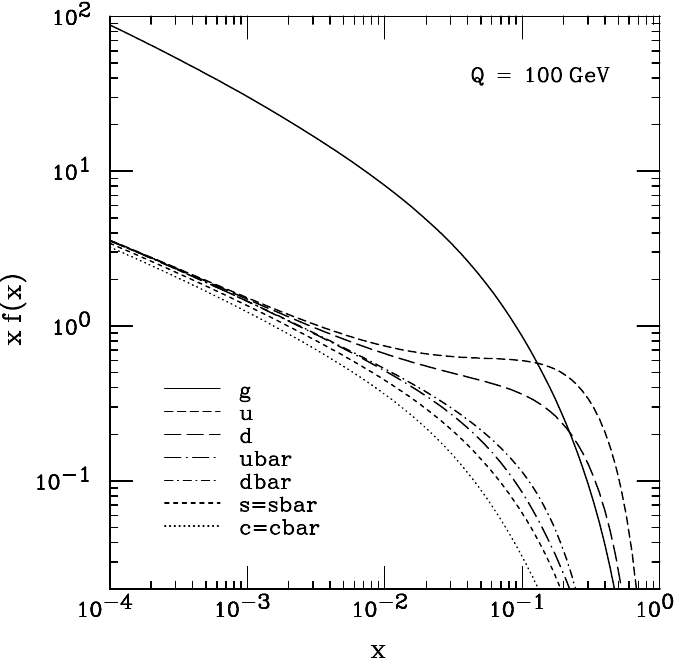
\includegraphics[width=0.42\textwidth]{./figs/CTEQ6M_pdf.png}
	\label{sfig:cteq6mpdf}
}
% \subfloat[Proton--(anti-)proton cross sections]{
% 	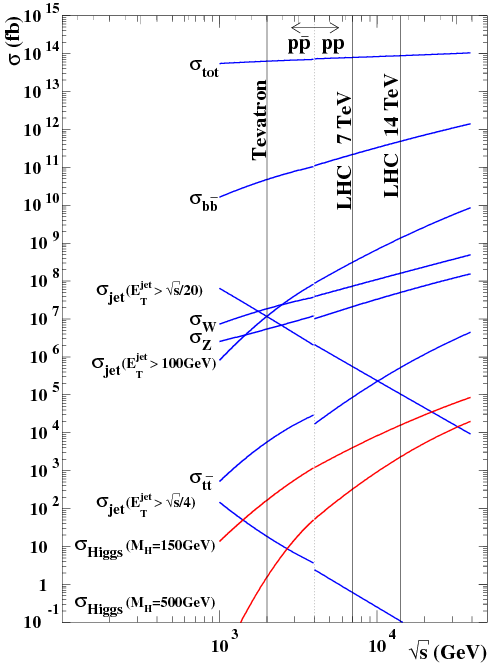
\includegraphics[height=0.55\textwidth]{./figs/figures_Theory_crosssections.png}
% 	\label{sfig:xsecs}
% }
\subfloat[Proton--proton cross sections]{
	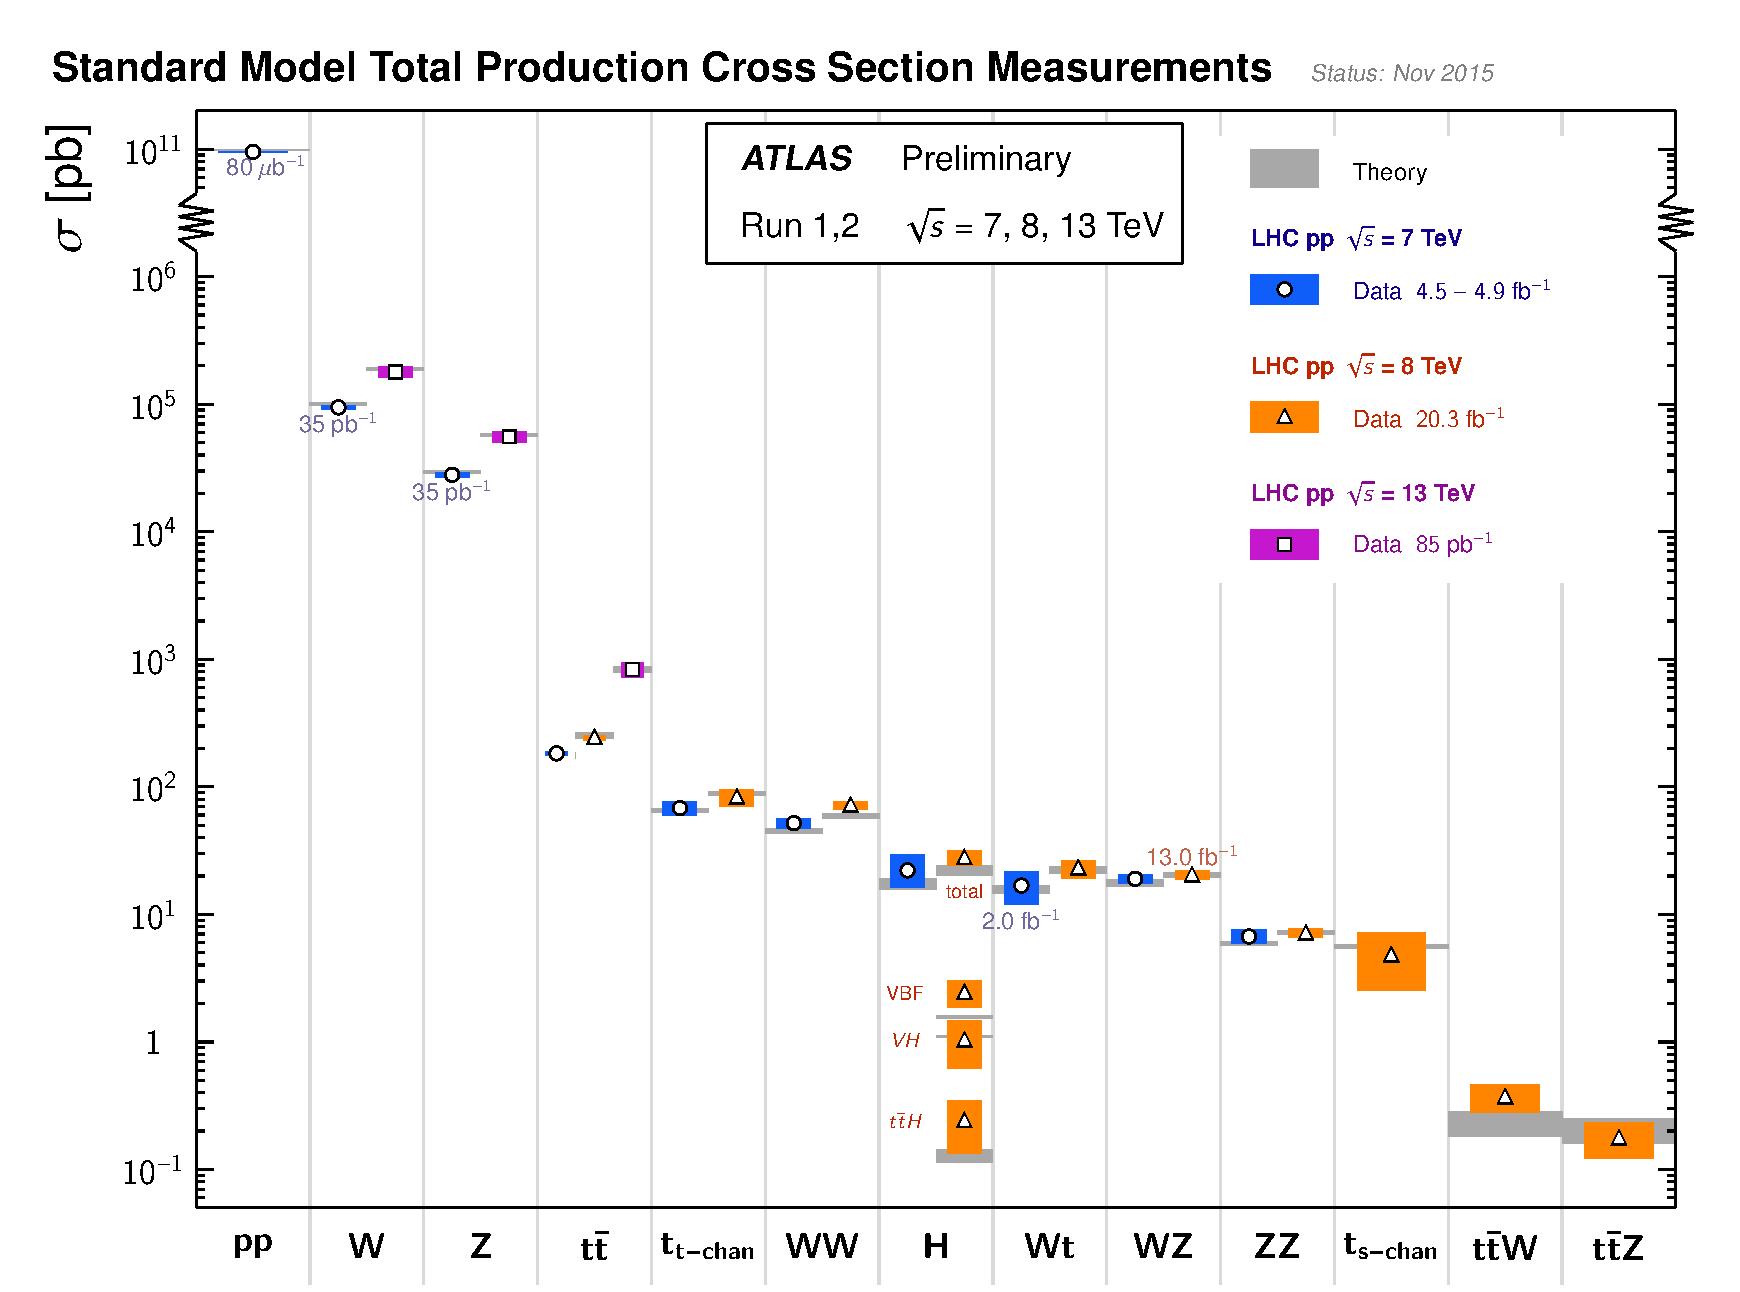
\includegraphics[width=0.58\textwidth]{./figs/ATLAS_a_SMSummary_TotalXsect.pdf}
	\label{sfig:xsecs}
}
\caption[Proton \gls{PDF} and cross section]{
\Fig~\subref{sfig:cteq6mpdf} shows the proton \gls{PDF} CTEQ6M~\cite{Pumplin2002}, evaluated at $\muf=Q=100~\GeV$. The lower $x$ regime is dominated by gluons.
%
\Fig~\subref{sfig:xsecs} shows the predicted and measured production cross section for \pp\ hard scattering for several final states including \ttbar\ at various \cmes~\cite{ATLASSMSummaryPlots}.
%
\label{fig:pdfxsec}}
\end{figure*}
%%%%%%%%%%%%%%%%%%%%%%%%%%%%%%%%%%%%%%%%%%%%%%%%%%%%%%%%%%%%%%%%%%%%%%%%%%%%%
%
%
At higher orders of perturbation theory, the partonic cross section is independent of the conveniently chosen factorisation scale \muf, which separates the two energy regimes. Divergences in perturbation theory are removed by a procedure referred to as renormalisation, which introduces another arbitrary scale \mur. For quick convergence, both scales are commonly chosen equal to the total momentum transfer $Q^2=\muf^2=\mur^2$. The total \tquark\ pair production cross section can then be formulated as:
%
\[
\sigma^{\ttbar}=
\sum_{i,j=q,\overline{q},g}\int \mathrm{d}x_{i} \mathrm{d}x_{j} f_{i}(x_{i},\muf^2) f_{j}(x_{j},\muf^2) 
\times 
[\alphas^2\sigma_0 (x_{i},x_{j},\sqrts) + \alphas^3(\mur^2)\sigma_1 (x_{i},x_{j},\sqrts)+ ...]_{{ij} \rightarrow \ttbar},
\]
%
with the sum running over possible all parton pairs $i$ and $j$ with momentum fractions $x_{i,j}$ of the original hadron. The functions $f_{i,j}$ are the hadron \glspl{PDF}, evaluated for the specific parton flavour and momentum fraction, as shown in \fig~\subref*{sfig:cteq6mpdf}. The values $\sigma_{0}$ and $\sigma_{1}$ denote the first two perturbative expansion coefficients of the partonic cross section in powers of \alphas, the coupling constant of the strong interaction. The cross section is shown for the three \pp collision \cmes\ of the \gls{LHC} in \fig~\subref*{sfig:xsecs}, together with other important processes. It rises from about $170$~\pb\ at $\sqrts=7$~\TeV\ to about $830$~\pb\ at $\sqrts=13$~\TeV~\cite{Czakon:2013goa}.%about 960 for 14 TeV

The dominant production mechanism for \tquark{s} at the \gls{LHC} is the pair production via gluon--gluon fusion, followed by quark--anti-quark annihilation. This can be seen from the momentum transfer requirement of the hard scatter for the production of a \tquark\ pair at rest, $Q^2 = s x_{i} x_{j} \geq 4 \mt^2$. Evaluated for $\sqrts=7~\TeV$, $\mt=175~\GeV$ and $x_1=x_2$, this yields $x$ values of about 0.05, for which the \gls{PDF} in \fig~\subref*{sfig:cteq6mpdf} reveals a dominant gluon contribution. The relevant lowest order Feynman diagrams are shown in \fig{s}~\subref*{sfig:ggfusion} and \subref{sfig:qqanni}. Due to the abundance and distinct final state of \tquark\ pair decays, measurements from \tquark\ pairs achieve highest precision in \tquark\ mass measurements and are in the focus of the analyses presented in this work. 
%
The other \tquark\ production mechanism is the \gls{EW} single \tquark\ production, which can be split into three processes, \Wboson--gluon fusion in the t-channel, $Wt$ production in the $Wt$ channel and quark--anti-quark annihilation in the s-channel, displayed in \fig{s}~\subref*{sfig:tchanfeyn}, \subref{sfig:Wtchanfeyn} and \subref{sfig:schanfeyn}, respectively. The total production cross sections for single \tquark\ processes at the \gls{LHC} are about a factor of $1/2$ lower than those for \ttbar\ production. Single \tquark\ events are used to directly probe the $Wtb$ vertex and measure the $V_{tb}$ element of the \gls{CKM} matrix.
%
%%%%%%%%%%%%%%%%%%%%%%%%%%%%%%%%%%%%%%%%%%%%%%%%%%%%%%%%%%%%%%%%%%%%%%%%%%%%%%%figures_Theory_LOProd.png
\begin{figure*}[tbp!]
\centering
% \subfloat[\Tquark\ pair production via gluon-gluon fusion or quark--anti-quark annihilation]{
% 	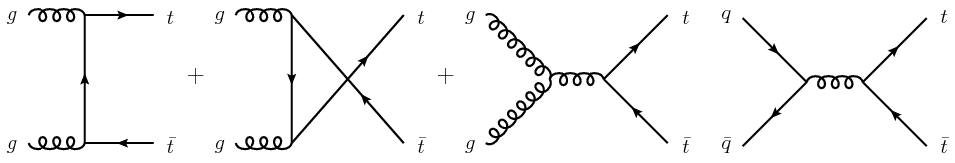
\includegraphics[width=0.9\textwidth]{figs/figures_Theory_LOProd_horizontal.png}
% 	\label{sfig:ttbarfeyn}
% }
% \\
% \subfloat[Single \tquark\ production in the t-, the $Wt$-and the s-channel]{
% 	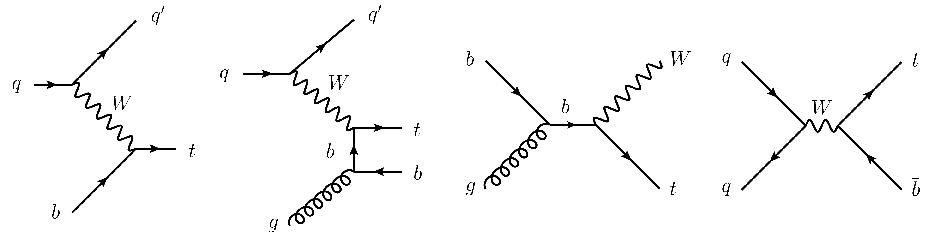
\includegraphics[width=0.9\textwidth]{figs/figures_Theory_LOProd_stop_horizontal.png}
% 	\label{sfig:stopfeyn}
% }
\subfloat[Gluon-gluon fusion]{
	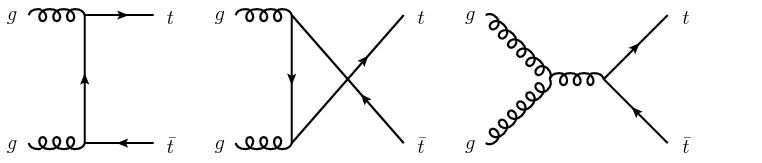
\includegraphics[height=0.15\textwidth]{figs/figures_Theory_LOProd_ggfusion.png}
	\label{sfig:ggfusion}
}
\subfloat[Quark--anti-quark annihilation]{
	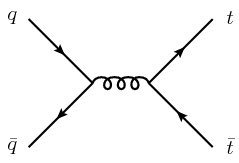
\includegraphics[height=0.15\textwidth]{figs/figures_Theory_LOProd_qqanni.png}
	\label{sfig:qqanni}
}
\\
\subfloat[t-channel, ]{
	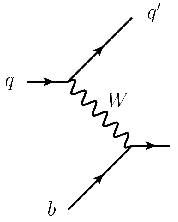
\includegraphics[height=0.15\textwidth]{figs/figures_Theory_stprod_tchan.png}
	\label{sfig:tchanfeyn}
}
\subfloat[$Wt$-channel]{
	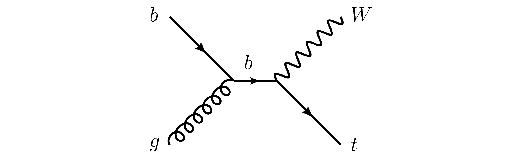
\includegraphics[height=0.15\textwidth]{figs/figures_Theory_stprod_Wt.png}
	\label{sfig:Wtchanfeyn}
}
\subfloat[s-channel]{
	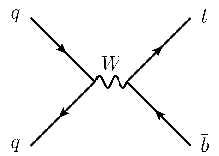
\includegraphics[height=0.15\textwidth]{figs/figures_Theory_stprod_schan.png}
	\label{sfig:schanfeyn}
}
\caption[Feynman diagrams for \tquark\ production]{
%
The lowest order Feynman diagrams of \ttbar\ production at hadron colliders via gluon fusion~\subref{sfig:ggfusion} and quark--anti-quark annihilation~\subref{sfig:qqanni}.
%
The \gls{EW} single \tquark\ production processes in the three production channels are shown below.
\label{fig:topprod}}
\end{figure*}
%%%%%%%%%%%%%%%%%%%%%%%%%%%%%%%%%%%%%%%%%%%%%%%%%%%%%%%%%%%%%%%%%%%%%%%%%%%%%
%








\subsection{Top quark decay}
%
Due to its high mass, the \tquark\ decays with a large decay width of about $1.4~\GeV$~\cite{PDG2014}. The corresponding lifetime is $\tau_t \approx 0.5 \times 10^{-24}$~s, which is too short, compared to the hadronisation time of $\tau_\mathrm{\gls{QCD}} \approx 1/\Lambda_\mathrm{\gls{QCD}} \approx 3 \times 10^{-24}$~s, for the \tquark\ to form toponium hadrons. 
%
The \tquark\ pair decay final state is classified according to the hadronic or leptonic decay of the two \Wboson{s} in the \ttbarll\ ($WW\rightarrow \ell \nu \ell \nu$), the \ttbarlj\ ($WW\rightarrow \ell \nu q q$) and the \ttbarjj\ ($WW\rightarrow q q q q$) channel. Using fermion universality in the \gls{LO} decay picture, the \Wboson\ can decay to nine different final fermion states, namely leptons of three and quarks of two different families, with the latter appearing in three different colour states. The \gls{LO} probability for a purely leptonic decay of the \ttbar\ pair is therefore $1/9=11.1\%$, to be compared with the experimental fraction of $10.3\%$~\cite{PDG2014}. The \ttbarlj\ and \ttbarjj\ channels  have a branching fraction of $43.5\%$ and $46.2\%$~\cite{PDG2014}, respectively. In analyses involving leptonic decay channels of the \ttbar\ pair, events containing tauonic decays are usually not considered, due to the intricate identification of hadronically decaying $\tau$ leptons. The branching fraction for the \ttbarll\ channel without $\tau$ intermediate states is about $5\%$. 


In addition to the \ttbar\ decay process, the initial state gluons and quarks can radiate gluons and thus contribute to the final state. This is referred to as \gls{ISR}.
%
The high energetic quarks and gluons from the \ttbar\ decay are then subject to gluon bremsstrahlung radiation, referred to as \gls{FSR}.
%
The following development of the state is characterised by subsequent gluon radiation, gluon splitting and quark pair production.
%
Due to the soft and collinear divergences, which appear in \gls{QCD} radiation, particles are radiated mostly in the direction of flight of the original parton, which leads to the development of a directed shower, referred to as a jet.
%
Coloured partons cluster to colour-singlet hadrons in a process referred to as hadronisation.
%
%
The physical objects present at this point interact with the detector and generate the experimentally observable final state, mainly consisting of photons, electrons, muons and jets. Their properties such as momentum, energy and charge can be measured. 
%
Neutrinos escape the detector without interaction and are therefore referred to as invisible. The momentum sum of all produced particles in the transverse direction to the beam adds up to zero. Consequently, the vector sum of the invisible particles' transverse momentum \pt\ shows up as \pt\ imbalance, referred to as missing transverse energy \met. Provided a sufficient detector acceptance, it is a measure for the transverse momentum sum of invisible particles.




\subsection{Top quark decay modelling}
%
The \ttbar\ decay modelling is usually performed at \gls{LO} or \gls{NLO} in perturbation theory, incorporated into a \gls{MC} generator program. The stage of the evolution after the subsequent \Wboson\ decays is commonly referred to as \genlevel. Since the distinction between decay stages is an artefact of numerical calculations, the exact definition of \genlevel\ depends on the \gls{MC} generator. This is treated in detail in \chap~\ref{chap:nlo}.
%
A \gls{PS} generator evolves the state further by successively applying the aforementioned \gls{QCD} radiation and conversion processes, until the energy scale of the hadronisation $Q_\mathrm{had}$ is reached. This arbitrary energy scale indicates the break-down of perturbation theory and is set following phenomenological observations, usually chosen as $Q_\mathrm{had} = \Lambda_{\gls{QCD}} \approx 200~\MeV$. For the hadronisation, two main phenomenological approaches are in use, the Lund--String model~\cite{Andersson198331,Andersson:1998tv}, based on expanding and breaking colour string fields and implemented in \Pythia, and the cluster fragmentation model~\cite{Webber:1983if}, implemented in the \Herwig\ program. The latter is based on the observation that parton configurations in a shower are independent of the starting energy scale, a phenomenon known as preconfinement. Both models sufficiently reproduce the experimental observations.
%
Following the hadronisation, the subsequent decay of unstable hadrons and leptons is the last stage of the \tquark\ decay modelling. This stage is commonly referred to as \stablevel, with stable particles defined as particles with a decay length of $c\tau>10$~mm~\cite{ATL-PHYS-PUB-2015-013}, corresponding to a life time of about $\tau>3\cdot10^{-11}$~s. 
%$3\times 10^{-10}$~s
This stage is well-defined and therefore often used for comparisons of \gls{MC} models, as detailed in \chap~\ref{chap:unfolding}. 
%
The full set of particles is then subject to a detector simulation, transforming the physical into the experimentally observable final state. This evolution stage is referred to as \recolevel\ and represents the frame for data to \gls{MC} comparisons and measurements like those presented in \chap{s}~\ref{chap:topmass7TeV} and \ref{chap:topmass8TeV}.






\section{The top quark mass}
%
Limited experimental precision on the \tquark\ mass \mt\ dominates the uncertainties of quantum loop corrections in \gls{QFT} calculations.
%
A precise knowledge of this parameter is crucial for many applications, such as the aforementioned \gls{EW} fits to assess the consistency of the \gls{SM}~\cite{Baak2014}. \Fig~\subref*{sfig:EWfit} shows the fitted contours at $68\%$ and $95\%$ confidence level in the \tquark\ and \Wboson\ mass plane, given the mass of the newly discovered \Hboson\ \mH. The intersection of the blue ellipsis with the one corresponding to the current world combination values for \mt\ and \mW\ in green shows the remarkable consistency of the \gls{SM}.
%
\Fig~\subref*{sfig:vacuumstability} shows that the \tquark\ mass is a key ingredient for the determination of the vacuum stability from the \Hboson\ quartic self-coupling~\cite{Degrassi2012}. Regions of stability in the \mt--\mH\ plane are marked in the phase diagram of the \gls{SM} \Hboson\ potential. The \gls{SM} appears to favour the meta-stable region at the boundary of stability and instability.
%
These and many more theoretical applications are the motivation for the large efforts, which have been put into a precise determination of the \tquark\ mass, leading to a current world combination value of $\mt = \XZtot{173.34}{0.76}~\GeV$~\cite{ATLAS:2014wva}.
%
%%%%%%%%%%%%%%%%%%%%%%%%%%%%%%%%%%%%%%%%%%%%%%%%%%%%%%%%%%%%%%%%%%%%%%%%%%%%%%%
\begin{figure*}[tbp!]
\centering
\subfloat[Consistency assessment of the \gls{SM} with an \gls{EW} fit]{
	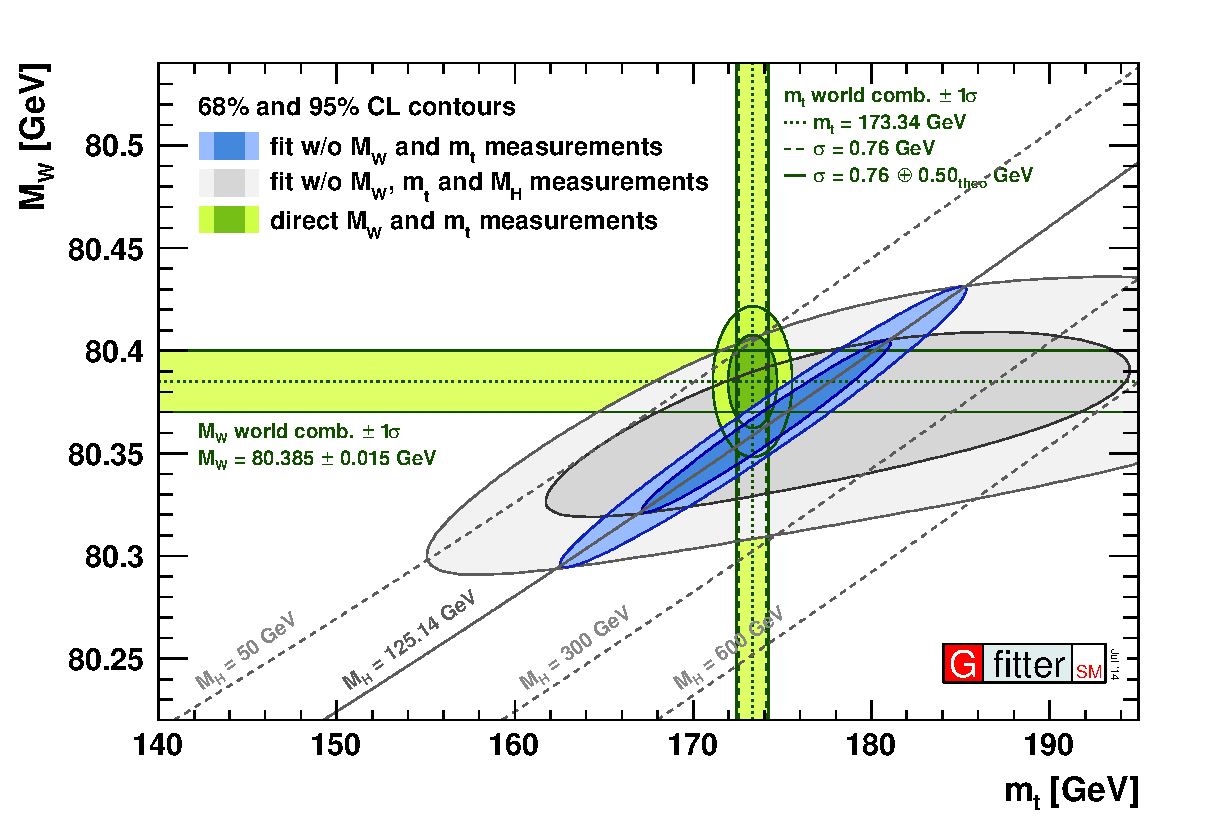
\includegraphics[height=0.40\textwidth]{figs/2014_07_16_Scan2D_MWvsmt_logo.eps}
	\label{sfig:EWfit}
}
\subfloat[Vacuum stability]{
	% \includegraphics[width=0.49\textwidth]{figs/deadoraliveG2012.pdf}
	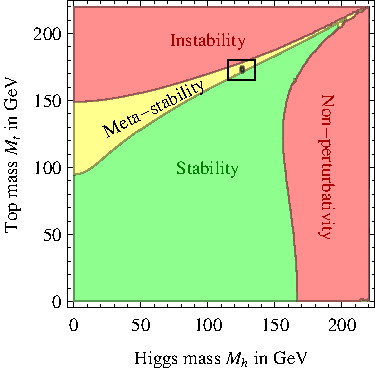
\includegraphics[height=0.38\textwidth]{figs/SMht.pdf}
	\label{sfig:vacuumstability}
}
\caption[Implications of the top quark mass]{
\Fig~\subref{sfig:EWfit} shows the fitted contours at $68\%$ and $95\%$ confidence level in the \mt\ and \mW\ plane, given the mass of the newly discovered \Hboson (blue ellipsis), in comparison with the current world combination values for \mt\ and \mW\ (green ellipsis)~\cite{Baak2014}.
%
\Fig~\subref{sfig:vacuumstability} shows the phase diagram of the \gls{SM} \Hboson\ potential and the vacuum stability as functions of \mt\ and \mH. The black dot denotes the position of the \gls{SM} vacuum in the meta-stable region~\cite{Degrassi2012}.
%
\label{fig:toprole}}
\end{figure*}
%%%%%%%%%%%%%%%%%%%%%%%%%%%%%%%%%%%%%%%%%%%%%%%%%%%%%%%%%%%%%%%%%%%%%%%%%%%%%










\subsection{Top quark mass definition}
\label{sect:topdefinition}
%
The precise knowledge of the experimental \mt\ parameter necessitates a careful definition of the term \tquark\ mass. 
%
Unlike, for example, the electron mass, the \tquark\ mass is not a physical observable, and the relation of the experimentally directly accessible quantity and the theoretically well-defined mass is still to be found. 
%
While experimentally, \mt\ is a quantity related to the invariant mass peak of the daughter particle system, theoretically, its definition depends on the mass scheme, chosen to optimise the convergence of the perturbative calculation. The most commonly used mass schemes are the pole mass scheme and the \gls{MSbar} scheme, related via a perturbative series in \alphas\ with an accuracy of $|\mtpole-\mtmsbar|  \leq \LambdaQCD \approx 200$~\MeV\ due to the renormalon ambiguity~\cite{Chetyrkin:1999ys,Melnikov:2000qh}.
%
The pole mass scheme is a long distance scheme, assuming asymptotically free final states, with \mt\ being defined as the real part of the perturbative \tquark\ propagator pole. 
%
% Given the short lifetime of \tquark{s} and colour confinement, this is a practical but not perfect assumption. On the calculational side, this is reflected by the absence of a pole in the scattering amplitude, since perturbation theory is simply a fixed order approximation of \gls{QCD}. 
% %
% The pole mass of the \tquark\ is therefore ill-defined when applied to problems outside perturbation theory. Additionally, perturbative corrections of the order of $\LambdaQCD \approx 200$~\MeV\ from the infinite sum of self-energy insertions have to be applied. This is known as the renormalon ambiguity~\cite{Beneke:1994sw,Beneke:1998ui}.
%
The \gls{MSbar} mass scheme is a short distance scheme, in which only divergent self-energy terms are absorbed into the mass parameter \mt. 
%
Both schemes show similar convergence of \mt\ up to \gls{NNLO}~\cite{Ahrens:2011px}.
%,Mangano_top2013
%
The \gls{MC} \gls{PS} programs incorporate phenomenological models of hadronisation and showering, including non-perturbative effects that in general prevent an unambiguous theoretical interpretation of the \tquark\ mass parameter.
%
Therefore, direct mass measurements effectively measure a \gls{MC} mass parameter without clear relation to any of the aforementioned schemes. Despite extensive research, the relation can only be estimated to be $|\mtpole-\mtMC| \leq 1~\GeV$~\cite{Buckley:2011ms,Hoang:2008xm,Agashe:2013hma,Juste:2013dsa,Skands:2007zg}.%,Mangano_top2013












\subsection{Top quark mass measurements}
\label{sect:TopQuarkMassMeasurements}

%
%%%%%%%%%%%%%%%%%%%%%%%%%%%%%%%%%%%%%%%%%%%%%%%%%%%%%%%%%%%%%%%%%%%%%%%%%%%%%%%
\begin{figure*}[tb!]
\centering
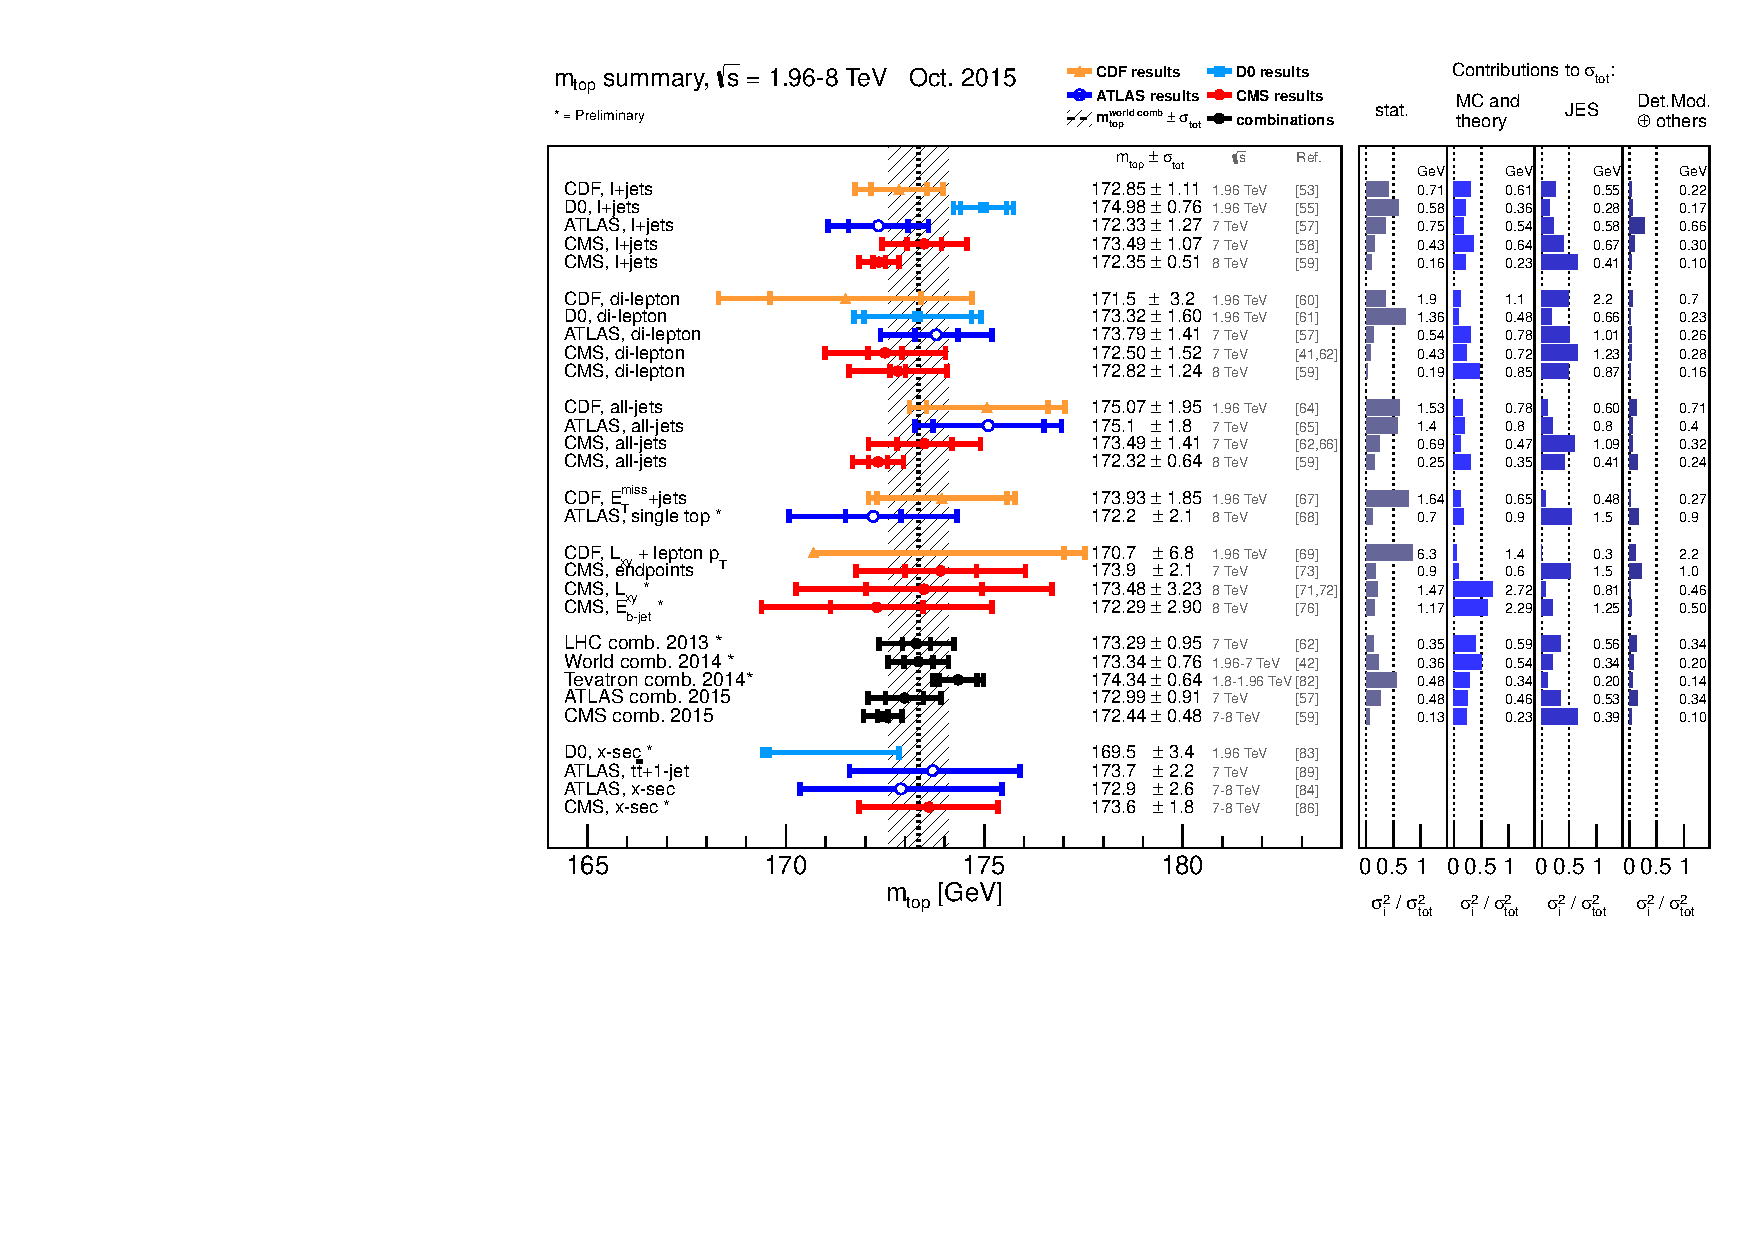
\includegraphics[width=0.99\textwidth]{./figs/mass_summary_sep2015.pdf}
\vspace{-0.3cm}
\caption[Summary of \mt\ measurements]{
%
Summary of the latest results of \gls{LHC} and Tevatron \mt\ measurements and their combinations, taken from \reference~\cite{Cortiana:2015rca}.
%
The central values and their symmetrised uncertainties are given on the left, compared to the result of the world combination~\cite{ATLAS:2014wva}. The columns on the right report the relative importance of the respective uncertainty categories on the total precision of the corresponding measurement.
%
\label{fig:mass_summary_sep2015}}
\vspace{-0.2cm}
\end{figure*}
%%%%%%%%%%%%%%%%%%%%%%%%%%%%%%%%%%%%%%%%%%%%%%%%%%%%%%%%%%%%%%%%%%%%%%%%%%%%%
%
The \tquark\ masses \mtpole\ and \mtMC\ are measured in various ways at the \gls{LHC}. A summary of the latest results of \gls{LHC} and Tevatron measurements and their combinations is given in \fig~\ref{fig:mass_summary_sep2015}. 

%direct
Direct \tquark\ mass measurements rely on the reconstruction of final states from detector objects and therefore assess the \mtMC\ mass. Various techniques are employed to match the reconstructed objects to the \gls{LO} decay hypotheses. This information can then either be used in a matrix element method to calculate a per event \gls{pdf} for \mt, formed by the convolution of \gls{LO} matrix elements and detector resolution functions, or for the comparison of experimental differential distributions to \gls{MC} predictions for different \mt\ hypotheses. The latter approach is computationally less demanding and therefore widely used, including the results presented throughout this work. The \mt\ sensitive quantities used therein are referred to as estimators. Results of direct \mt\ measurements and their combinations are shown in the top four and the second to last group of \fig~\ref{fig:mass_summary_sep2015}, respectively.


%indirect
Indirect \tquark\ mass determinations use the theoretically predicted and the experimentally determined total or differential \ttbar\ production cross section as a function of \mt. The \tquark\ mass information is drawn from the intersection of both curves. Since  with the latest improved event selections experimentally determined cross sections rely only marginally on \mtMC, this approach can provide a measurement of \mtpole~\cite{Nisius:2012gm}.
%
However, it still suffers from large uncertainties, mostly limited by \gls{PDF} and scale uncertainties and the precision of the integrated luminosity and beam energy determinations~\cite{ATLASCollaboration2014a,CMS-PAS-TOP-13-004}. Further reduction of uncertainties will require considerable efforts on both the theoretical and the experimental side.
%
A measurement of the \mtpole\ mass has also been performed using \ttbarj\ events, by comparing the normalised differential cross section calculations at \gls{NLO} precision in \gls{QCD} to data at \genlevel, corrected for detector effects with an unfolding procedure~\cite{ATLAS:2014zza}. The measurement exploits the dependence of gluon radiation on \mt\ and reaches a final precision compatible with the one from the aforementioned cross section approach. In contrast to the analysis from the cross-section, this measurement is presently statistically limited and will therefore profit from the large amount of data to be collected during future operation of \gls{LHC}.
%
% A relatively new idea is the construction of two measurements with maximal correlation, a direct and an indirect one to determine \mtMC\ and \mtpole\ at the same time. These two measurements have to be constructed largely correlated, such that, irrespective of their total uncertainty, the uncertainty of the difference in central \mt\ values, $\mtpole-\mtMC$, is small. The challenge in this approach is to maintain the high correlation throughout the full analysis procedure. This is currently investigated at \gls{ATLAS}, using the \tquark\ mass measurement in the \ljets\ channel, presented in \sect~\ref{sec:ljanalysis7TeV} and documented in \reference~\cite{Aad:2015nba}, and the aforementioned measurement of \mtpole\ at \genlevel. 
%
Indirect \mt\ determination results are shown in the lowest group of \fig~\ref{fig:mass_summary_sep2015}.

%alternative
\Tquark\ mass measurements, using other than the traditional techniques described above, are referred to as alternative measurements. Various \mt\ dependent observables are exploited, such as kinematic endpoints\cite{CMSCollaboration2013a} or the \bhadron\ Lorentz boost via its decay length~\cite{CMSCollaboration2013}. These measurements still suffer from relatively large statistical and systematic uncertainties and are therefore presently only conceptually valuable.
%
Alternative \mt\ measurement results are shown in the fifth group of \fig~\ref{fig:mass_summary_sep2015}.




